%!TEX root = karulf-thesis.tex
\chapter{User Study}
We conducted a formal user study to evaluate the effectiveness of the RIDE interface and test the validity of our thesis. We designed an hour long user study with the goal of testing the asynchronous task and notification system.

We conducted a two-condition experiment, one with notification displayed and one with notifications hidden. An example notification is shown in Figure~\ref{fig:notification}. 

The user study was advertised via flyers posted publicly on the Washington University Campus. Our user pool consisted of 22 adult participants, 6 female and 16 male, approximately 23.50 years of age ($\sigma=5.45$).

We ran each participant individually through a the user study session. A user study session consisted of a pre-experiment questionnaire, a short set of practice sessions, two search and rescue experiments, and a post-experiment questionnaire. We created two separate experiment conditions, one without notifications and one with notifications, and created a program to execute both in a random order during the user study. The testing procedures will be described in more detail in the Section~\ref{testing}.

Unfortunately, there were several fundamental flaws in the design of the user studies that prevent us from clearly rejecting the null hypothesis. I will briefly discuss the results of the user study in Section~\ref{results}. Finally in Section~\ref{conclusion} I identify several shortcomings of the current user study design. In Section~\ref{futurework} on future work, I propose several modifications to the user study that address the shortcomings of this research.

\section{Experimental Design}
The goal of our user studies was to determine if the RIDE user interface was an effective tool for control groups of robots. Our secondary goal was to test the individual interface elements unique to RIDE to determine if they enhanced the user experience. We looked through prior work to find activities that a group of robots could accomplish more effectively if controlled properly and would not require background experience. We decided upon ``search and rescue'' as it is a generally understood activity that can be accomplished faster through effective coordination of robots. 

We designed a scenario where the robots were used to find boxes hidden throughout a house. The boxes would not be visible on the on-screen map directly, but they would display through the sensors on the robots. The house can be seen, without boxes, in Figure~\ref{fig:test-environment}. 

\begin{figure}[ht]
\begin{center}
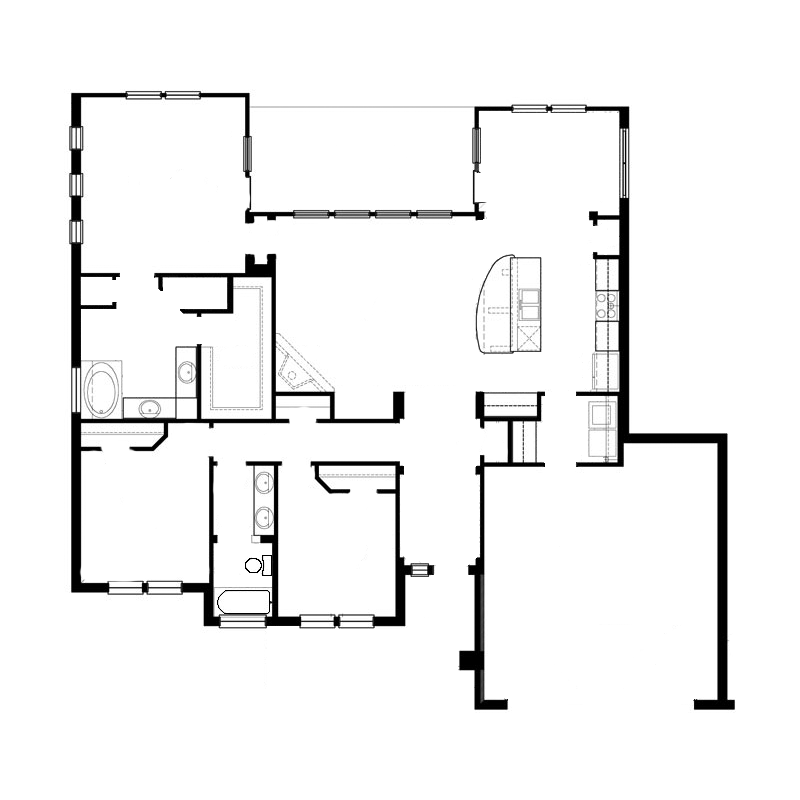
\includegraphics[width=5in]{images/generic-house.png}
\caption{User Testing Environment\label{fig:test-environment}}
\end{center}
\end{figure}

The robots were configured to simulate Erratic ERA-MOBI robots. The simulation engine, as described in Section~\ref{sub:simulator}, was programmed to emulate a laser sensor and an odometry sensor. These two sensors allowed the robot to detect the boxes, walls, and other obstacles through the laser readings or by picking up a stalled engine through the odometry sensor.

We designed three separate runs for a user study session: a training run, a run with notifications disabled, and a run with notifications enabled. We decided to assume that users would have a small amount of training before they were allowed to control robots. In order to meet this assumption, we provided each user with the same practice run to ensure a common training set.

In the following subsections I will describe, in order, the components of a user study session. This research protocol was approved by the Washington University Institutional Review Board (IRB). The full documentation submitted to the IRB including the user study script may be found in Appendix~\ref{app:IRB}.

\subsection{Pre-Experiment} % (fold)
\label{sub:pre_experiment}
The first step to each user study session is obtaining informed consent for participation in human subjects research. The informed consent paperwork may be found in Appendix~\ref{app:IRB}. Once consent had been obtained, the user was asked to fill out a short pre-experiment questionnaire. The goal of the questionnaire was to obtain useful information for correlating in data analysis. We asked for background information such as computer use, video game experience, and robotics experience.

Once the user had filled out the questionnaire, regardless of experience the user was given a short lecture on robotics. We decided that target audience for RIDE would have a basic understanding of the robots they were controlling. The lecture covered basic concepts including robot movement (quasi-holonomic  vs holonomic) and laser range finders.

After a scripted lecture on robotics we ask the user to narrate their thought process out loud, a practice called ``speak aloud'' within the HCI community. We ask the user to play a round of minesweeper while speaking their thoughts out loud to practice speaking out-loud. The pre-experiment preparation concludes when the researcher is confident in the participants ability to describe their thought process.
% subsection pre_experiment (end)

\subsection{Training Run} % (fold)
\label{sub:training_run}
The training run takes place inside the virtual house pictured in Figure~\ref{fig:test-environment}. Unlike the experimental runs there are no boxes located within the house during the training run. Instead the user is asked to demonstrate basic control over the interface by accomplishing a series of tasks. The full transcript of the user study - including the checklist of required skills to complete the training run - is found in Appendix~\ref{app:IRB}. Once the user completed the training activities they are given an opportunity to continue using the user interface until they feel comfortable proceeding to the experiments.
% subsection training_run (end)

\subsection{RIDE UI Experiments} % (fold)
\label{sub:ride_ui_experiments}
The user study program randomly chooses either the notification or the non-notification experiment. In both experiments, participants were told of four boxes hidden within the house. We asked participants to find the boxes quickly. Once a user believed they had found box they were instructed to circle the box with their mouse pointer. This information was used in conjunction with other data in post-processing to determine if the user correctly identified each box.

During the experiment, the researcher was unable to offer any advice or answer any questions. The researcher took hand-written notes on each experiment with an emphasis on recording information related to the user's thought process. The automated user study application is set to record keystrokes, mouse events, application state and the screen of the participant.

% subsection ride_ui_experiments (end)

\subsection{Post-Experiment} % (fold)
\label{sub:post_experiment}
We asked participants a series of structured and semi-structured questions to conclude the user study. The post-experiment questionnaire can be found in Appendix~\ref{app:IRB}.

We also conducted a brief semi-structured interview after the post-experiment questionnaire. These questions were based off of remarkable events noted by the researcher during the experiments. The semi-structured interview results were not included in formal analysis of RIDE, rather they were aimed to provide insight for continued application development.
% subsection post_experiment (end)
